%%% See example_beamer.tex for a more detailed example.
\documentclass[t,xcolor=table,english]{beamer}   %% ngerman, german, english
\usepackage[utf8]{inputenc}        
%% Umlautkodierung UTF-8
%\usepackage[latin1]{inputenc}         %% Umlautkodierung Latin-1
\usetheme{wiaspr}

\begin{document}

\title{Optimal Shape Design of Air Ducts in Combustion Engines}
\author{Hong Nguyen}
\date{\today}

\wiasGroup*{1}{FG8}
\wiasTitleSlide

\section[General]{General}
\begin{frame}
	\frametitle{\href{https://www.romsoc.eu/optimal-shape-design-of-air-ducts-in-combustion-engines/}{ROMSOC Project 11}}
	\textbf{General Information.}
	\begin{itemize}
		\item Within the \textit{European Innovative Training Network} (ITN): \href{https://www.romsoc.eu/}{Reduced Order Modeling, Simulation and Optimization of Coupled Systems} (ROMSOC).
		\item \textit{Project 11}: \href{https://www.romsoc.eu/optimal-shape-design-of-air-ducts-in-combustion-engines/}{Optimal Shape Design of Air Ducts in Combustion Engines}.
		\item \textit{Project Partners}: \href{https://www.wias-berlin.de/}{WIAS}, Germany; \href{https://mathtec.at/}{Math.Tec} GmbH, Austria.
		\item \textit{Starting Date}: Mar 16, 2020. \textit{Contract}: 17.5 months, extension in the network is potentially possible (6 months); some additional months. 
		\item To be discussed: Total 8 months in Austria (Date not yet specified); Ethics.
		\item Next Delivery: D5.3 - Software with benchmark problems.
	\end{itemize}
	\textbf{Training Process.} 
	\begin{itemize}
	\item \textit{Canceled}: \href{https://www.jyu.fi/en/research/summer-and-winter-schools/jss/courses/courses-in-mathematics}{Jyv\"askyl\"a Summer School}, Finland; \href{https://www.applied.math.tugraz.at/tagungen/samm20/}{SAMM 2020} in Graz, Austria.
	\item \textit{Waiting}: \href{http://www.wias-berlin.de/events/TESenergy/\#studentcompactcourse}{Student Compact course, Thematic Einstein Semester}, TU Berlin.
	\item \textit{On going}: Stephan Schmidt's Shape Optimization Course, HU.
	\item \textit{Winter term}: Topology Optimization.
\end{itemize}
\end{frame}

\begin{frame}
	\frametitle{Up to Now}
	\textbf{Theory.}
	\begin{itemize}
		\item Gather literature on: Shape Optimization, NSEs, (not yet on Turbulence).
		\item Get familiar with:
		
		- \textit{NSEs} [Temam2000, Maz'ya-Rossmann2009];
		
		- \textit{Shape Optimization} [Schmidt2020, Sokolowski-Zol\'esio1992];
		
		- \textit{Turbulence Models} $k$-$\epsilon$ [Mohammadi-Pironneau1994].
		\item Read [Temam2000]: NSEs with Dirichlet BCs in Lipschitz domains.
		\item Read [Maz'ya-Rossmann2009] for polygonal domains and {\color{red} general mixed BCs}, existence (fixed-point argument).
	\end{itemize}
	\textbf{Numerics.}
	\begin{itemize}
		\item Martin Kanitsar's code runs $\approx 2$ days for 6 gradient descent steps.
		\item Installation of software: {\color{red} OpenFOAM} (latest), additionally: FEniCS, Fireshape (on Firedrake, AD)[Paganini-Wechsung], AD, ROL.
		\item Started 2 Documentations: Understand Kanitsar's codes + Relevant parts of OpenFOAM.
	\end{itemize}
\end{frame}

\begin{frame}
	\frametitle{Next Steps}
	\textbf{Theory.}
	\begin{itemize}
		\item Learn Shape and Adjoint Calculus.
		\item Literature on: {\color{blue} turbulence/turbulent + adjoint}
		\begin{itemize}
			\item Hartmann, Ralf; Held, Joachim; Leicht, Tobias. \textit{Adjoint-based error estimation and adaptive mesh refinement for the RANS and $k$-$\omega$ turbulence model equations}. J. Comput. Phys. 230 (2011), no. 11, 4268-4284.
			\item Vishnampet, Ramanathan; Bodony, Daniel J.; Freund, Jonathan B. \textit{A practical discrete-adjoint method for high-fidelity compressible turbulence simulations}. J. Comput. Phys. 285 (2015), 173–192.
			\item Marta, Andre C.; Shankaran, Sriram. \textit{On the handling of turbulence equations in RANS adjoint solvers}. Comput. \& Fluids 74 (2013), 102–113.
			\item Kavvadias, I. S.; Papoutsis-Kiachagias, E. M.; Dimitrakopoulos, G.; Giannakoglou, K. C. The continuous adjoint approach to the $k$-$\omega$ SST turbulence model with applications in shape optimization. Eng. Optim. 47 (2015), no. 11, 1523–1542. \ldots
		\end{itemize}		
		\item Analyze the existence of optimization problems.
		\item Learn Turbulence ($k$-$\epsilon$).
		\item Topology Optimization (TO).
	\end{itemize}
	\textbf{Numerics.}
	\begin{itemize}
		\item Learn OpenFOAM; Upgrade Martin Kanitsar's Code (2012) to latest version of OpenFOAM (considerable difference before/after 2016). 
	\end{itemize}
\end{frame}

\begin{frame}
	\frametitle{Targets}
	\textbf{Theory.}
	\begin{itemize}
		\item \textit{1st Target}: Implementation of Shape Optimization on Semi-discrete NSEs in 3D + Turbulence.
		\begin{align*}
		\frac{{\bf v}^{n+1} - {\bf v}^n}{\Delta t} - \nu\Delta{\bf v}^{n+1} + ({\bf v}^{n+1}\cdot\nabla){\bf v}^{n+1} + \nabla p^{n+1} = {\bf f}^{n+1} \mbox{ in } \Omega,\ n = 1,\ldots,N.
		\end{align*}
		\item Continuous adjoint + Theoretical framework.
		\item Implementation of continuous adjoint and turbulence.
	\end{itemize}
	\textbf{Software.}
	\begin{itemize}
		\item Upgrade Software (e.g. OpenFOAM) to latest version. 
		\item 2D version of codes.
		\item Replace Star-CCM+.
		\item Time-dependent case.
	\end{itemize}
\end{frame}

\begin{frame}
	\frametitle{Mathematical Theory: A Roadmap}
	\begin{itemize}
		\item In order to model the flow in the considered shape, use the stationary NSEs for the \textit{velocity} ${\bf v}$ and the \textit{kinematic pressure} $p$:
		\begin{equation}
		\label{NSEs1}
		\tag{NSEs1}
		\left\{\begin{split}
		- \nu\Delta{\bf v} + ({\bf v}\cdot\nabla){\bf v} + \nabla p &= {\bf f} \mbox{ in } \Omega,\\
		\nabla\cdot{\bf v} &= 0 \mbox{ in } \Omega,\\
		{\bf v} &= {\bf f}_{\rm i} \mbox{ on } \Gamma_{\rm i},\\
		{\bf v} &= {\bf 0} \mbox{ on } \Gamma_{\rm w},\\
		{\color{red}-\nu\partial_{\bf n}{\bf v} + p{\bf n}} &= {\bf 0} \mbox{ on } \Gamma_{\rm o},
		\end{split}\right.
		\end{equation}
		where ${\bf f}_{\rm i}$ is the \textit{inflow profile}, $\nu$ is the \textit{viscosity}, and ${\bf n}$ is the outer normal vector.
		\item \textbf{Weak formulation.} $({\bf v},p)\in W^{1,2}(\Omega)^3\times L^2(\Omega)$ satisfying
		\begin{align*}
		\nu\int_\Omega \nabla{\bf v}:\nabla{\bf w} + \int_\Omega ({\bf v}\cdot\nabla){\bf v}\cdot{\bf w} - \int_\Omega p\nabla\cdot{\bf w} &= \int_\Omega {\bf f}\cdot{\bf w},\ \forall{\bf w}\in V,\\
		\nabla\cdot{\bf v} = 0 \mbox{ in } \Omega,\ {\bf v} = {\bf f}_{\rm i} \mbox{ on } \Gamma_{\rm i},\ {\bf v} &= {\bf 0} \mbox{ on } \Gamma_{\rm w}.
		\end{align*} 
		\item (Not yet) {\color{blue} Existence of Optimal Shape.}
		\item (Not yet) {\color{blue} Shape Derivative and Optimality Condition; 2 Formulations: Domain and Boundary.}
		\item Laplace Beltrami smoothing, Geometrical constraints.
	\end{itemize}
\end{frame}

\begin{frame}
	\frametitle{2nd BVP for NSEs}
	\begin{itemize}
		\item A particular relevant case of [Maz'ya-Rossman2009]:
		\begin{equation}
		\label{NSEs mixed BCs}
		\tag{NSEs2}
		\left\{\begin{split}
		- \nu\Delta{\bf v} + ({\bf v}\cdot\nabla){\bf v} + \nabla p &= {\bf f} \mbox{ in } \Omega,\\
		{\color{red}-\nabla\cdot{\bf v}} &= g \mbox{ in } \Omega,\\
		{\bf v} &= {\bf f}_{\rm i} \mbox{ on } \Gamma_{\rm i},\\
		{\bf v} &= {\bf 0} \mbox{ on } \Gamma_{\rm w},\\
		{\color{red}-2\nu\varepsilon_{\bf n}({\bf v}) + p{\bf n}} &= {\bf 0} \mbox{ on } \Gamma_{\rm o},
		\end{split}\right.
		\end{equation}
		\item \textbf{Weak formulation.} $({\bf v},p)\in W^{1,2}(\Omega)^3\times L^2(\Omega)$ satisfying
		\begin{align*}
		b({\bf v},{\bf w}) + \int_\Omega ({\bf v}\cdot\nabla){\bf v}\cdot{\bf w}dx - \int_\Omega p\nabla\cdot{\bf w}dx &= \int_\Omega {\bf f}\cdot{\bf w}dx,\ \forall {\bf w}\in V,\\
		\nabla\cdot{\bf v} = 0 \mbox{ in } \Omega,\ {\bf v} = {\bf f}_{\rm i} \mbox{ on } \Gamma_{\rm i},\ {\bf v} &= {\bf 0} \mbox{ on } \Gamma_{\rm w},
		\end{align*}
		where $V := \{{\bf v}\in W^{1,2}(\Omega)^3;{\bf v} = {\bf f}_{\rm i} \mbox{ on } \Gamma_{\rm i},\ {\bf v} = {\bf 0} \mbox{ on } \Gamma_{\rm w}\}$, and
		\begin{align*}
		b({\bf v},{\bf w}) := 2\nu\int_\Omega \sum_{i,j = 1}^3 {\color {red}\varepsilon_{ij}({\bf v})\varepsilon_{ij}({\bf w})}dx \mbox{ where } {\color{red}\varepsilon_{ij}({\bf v}) := \frac{\partial_{x_i}v_j + \partial_{x_j}v_i}{2}}.
		\end{align*}
	\end{itemize}	
\end{frame}

\begin{frame}
	\frametitle{Existence Theorem}
	\begin{theorem}[Maz'ya-Rossman2009]
		\textbf{Assumptions.}
		\begin{itemize}
			\item ${\bf f}_{\rm i}\in W^{1/2,2}(\Gamma_{\rm i})^3$ s.t. $\exists {\bf w}\in W^{1,2}(\Omega)^3$ satisfying the conditions ${\bf w}|_{\Gamma_{\rm i}} = {\bf f}_{\rm i}$ and ${\bf w}|_{\Gamma_{\rm w}} = {\bf 0}$.
			\item Suppose that $L_V := \{w\in V;\varepsilon({\bf w}) = {\bf 0}\} = \{{\bf 0}\}$ and $\|{\bf f}\|_{V^\star} + \|{\bf f}_{\rm i}\|_{W^{1/2,2}(\Gamma_{\rm i})^3}$ is sufficiently small.
		\end{itemize}
		\textbf{Existence.} Then there exists a solution $({\bf v},p)\in W^{1,2}(\Omega)^3\times L^2(\Omega)$ of \eqref{NSEs mixed BCs}.
		\textbf{Uniqueness.}
		\begin{itemize}
			\item ${\bf v}$ is unique on the set of all functions with norm $<$ a certain $\varepsilon > 0$.
			\item $p$ is unique (due to the BC on $\Gamma_{\rm o}$).
		\end{itemize}
	\end{theorem}
\end{frame}

\begin{frame}
	\frametitle{Cost Functional}
	\textbf{Main Problem.} Find an $\Omega\in\mathcal{O}_{\rm ad}$ s.t. 2 criteria are considered:
	\begin{itemize}
		\item \textbf{Uniform Outflow Criteria.} The normal component of the outflow ${\bf v}\cdot{\bf n}|_{\Gamma_{\rm o}}$ should be close to uniform on entire $\Gamma_{\rm o}$.
		
		By conservation of mass, the average outflow is $\overline{v} = \frac{1}{|\Gamma_o|} \int_{\Gamma_i} - {\bf f}_i\cdot {\bf n}$. Consider:	
		\begin{align*}
		\mathcal{J}_1({\bf v}(\Omega)) := \frac{1}{2}\int_{\Gamma_o} ({\bf v}\cdot {\bf n} - \overline{v})^2.
		\end{align*}
		\item \textbf{Total Pressure Loss Criteria.} Bernoulli principle: The total pressure $p + \frac{1}{2}|{\bf v}|^2$ is a quantity that remains constant along the streamlines.
		
		Minimize the drop of pressure from $(p + \frac{1}{2}|{\bf v}|^2)|_{\Gamma_{\rm i}} > (p + \frac{1}{2}|{\bf v}|^2)|_{\Gamma_{\rm o}}$. Consider:
		\begin{align*}
		\mathcal{J}_2(({\bf v},p)(\Omega)) := -\frac{|\Gamma_i|}{|\Gamma_i^\varepsilon|} \int_{\Gamma_i^\epsilon}\left(p + \frac{1}{2}|{\bf v}|^2\right){\bf v}\cdot {\bf n} - \frac{|\Gamma_o|}{|\Gamma_o^\varepsilon|}\int_{\Gamma_o^\varepsilon} \left(p + \frac{1}{2}|{\bf v}|^2\right){\bf v}\cdot {\bf n}.
		\end{align*}
	\end{itemize}
\end{frame}

\begin{frame}
	\frametitle{Mixed Cost Functional}
	\begin{align}
	\label{J12}
	\tag{$\mathcal{J}_{12}$}
	\mathcal{J}_{12}({\bf v}(\Omega)) := (1 - \gamma)\mathcal{J}_1({\bf v}(\Omega)) + \gamma\rho\mathcal{J}_2({\bf v}(\Omega)),
	\end{align}
	with the \textit{weighting parameter}  $\gamma \in [0,1]$ and (not yet considered)
	\begin{equation*}
	\rho := \left\{\begin{split}
	&\frac{\|\partial \mathcal{J}_1({\bf v}(\Omega^0))\|_{L^2(\Gamma_w^0)}}{\|\partial \mathcal{J}_2({\bf v}(\Omega^0))\|_{L^2(\Gamma_w^0)}} &\mbox{ if } \gamma \in (0,1),\\
	&1 &\mbox{ if } \gamma\in \{0,1\}.
	\end{split}\right.
	\end{equation*}
\end{frame}

\begin{frame}
	\frametitle{OpenFOAM's Structure}
	OpenFOAM layout constitutes of 2 main directories:
	\begin{itemize}
		\item \texttt{OpenFOAM-<version>}:   OpenFOAM libraries
		\item \texttt{ThirdParty}: A set of third-party libraries.
	\end{itemize}
	\textbf{OpenFoam Cases.} configured by several plain text input files in 3 directories:
	\begin{itemize}
		\item \texttt{0/}: initial time directory including field files.
		\item \texttt{system/}: \texttt{controlDict, fvSchemes, fvSolution}
		\item \texttt{constant/}: \texttt{polyMesh/}, and files declaring constant values.
	\end{itemize}
	\textbf{OpenFOAM Solvers.}
	\begin{itemize}
		\item \texttt{Make/}: \texttt{files} (declare the main C++ file and its location to generate dependencies), \texttt{options} (include OpenFOAM libraries).
		\item \texttt{createFields.H}: Declare types of all variables needed.
		\item \texttt{<Solver-Name>.C}: Main script declared in \texttt{Make/}.
	\end{itemize}
\end{frame}

\begin{frame}
	\frametitle{Outputs of Martin Kanitsar's Codes}
	\begin{figure}
		\centering
		\includegraphics[scale=0.4]{Compare_Tubes}
		\caption{Left: Initial Tube. Right: Optimized Tube after 6 Gradient-Descent Iterations.}
	\end{figure}
\end{frame}

\begin{frame}
	\frametitle{Values of Cost Functional $\mathcal{J}_{12}$}
	Choose the weighting parameter $\gamma = 1$ (\texttt{dp\_J12} in Martin Kanitsar's code), so $\rho = 1$:
	
	\begin{table}
		\centering
		\begin{tabular}{|c|l|l|l|}
			\hline
			\textbf{Iteration} & $(1 - \gamma)\mathcal{J}_1$ & $\gamma\mathcal{J}_2$ & $\mathcal{J}_{12}$ \\
			\hline
			0 & 0 & 181.731920964434 & 182.07227883754 \\
			\hline
			1 & 0 & 180.335741264281 & 180.929940529294 \\
			\hline
			2 & 0 & 179.204741499965 & 180.136772627044 \\
			\hline
			3 & 0 & 178.618996623167 & 179.571215644196 \\
			\hline
			4 & 0 & 177.72661280195 & 179.091345594335 \\
			\hline
			5 & 0 & 176.968052608864 & 178.804927417778 \\
			\hline
			6 & 0 & 176.187919434572 & 178.048912220916 \\
			\hline
		\end{tabular}
	\end{table}
	\textbf{Q}: \textit{Why $\mathcal{J}_{12}\ne(1 - \gamma)\mathcal{J}_1 + \gamma\rho\mathcal{J}_2$?}
\end{frame}

\begin{frame}
	\frametitle{FEniCS}
	\textbf{Example.} Incompressible NSEs for flow around a cylinder:
	\begin{align*}
	{\bf v}_t + ({\bf v}\cdot\nabla){\bf v} - \nabla\cdot(\sigma({\bf v},p)) = {\bf f},\ \nabla\cdot{\bf v} = 0,
	\end{align*}
	with $T = 5$, $dt = 10^{-3}$, $\mu = 0.5$, $\rho = 1$.
	\begin{figure}
		\centering
		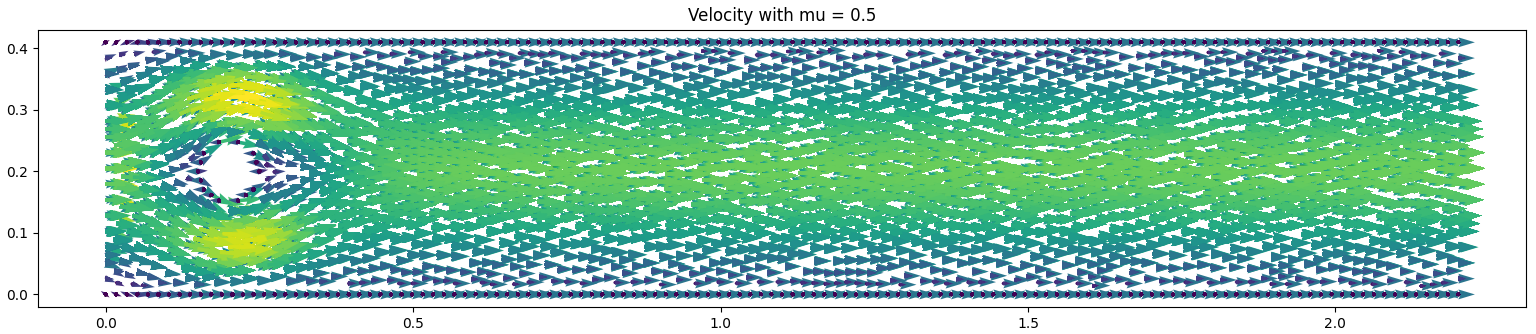
\includegraphics[width=\textwidth]{Velocity_05}
	\end{figure}

	\begin{figure}
		\centering
		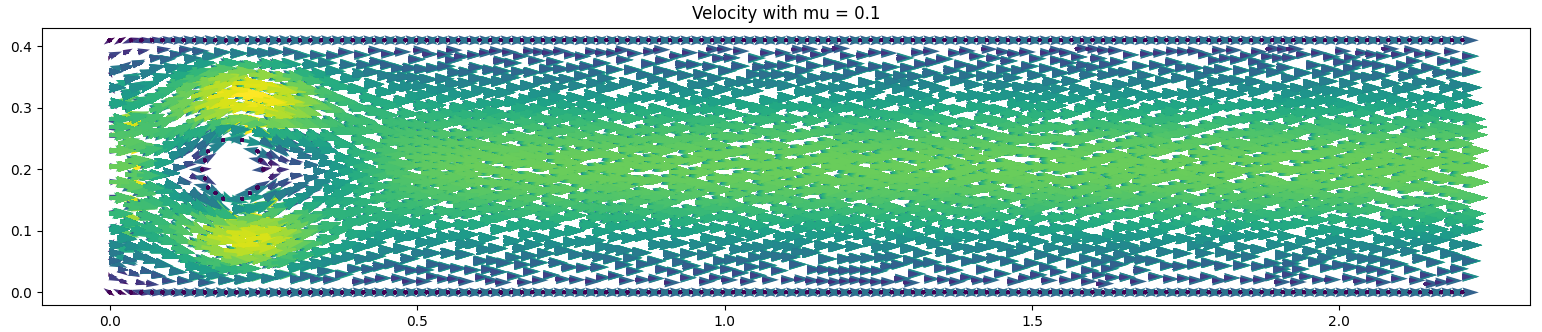
\includegraphics[width=\textwidth]{Velocity_01}
	\end{figure}
\end{frame}

\begin{frame}
	\frametitle{Velocities with Different Viscosities}
	\begin{figure}
		\centering
		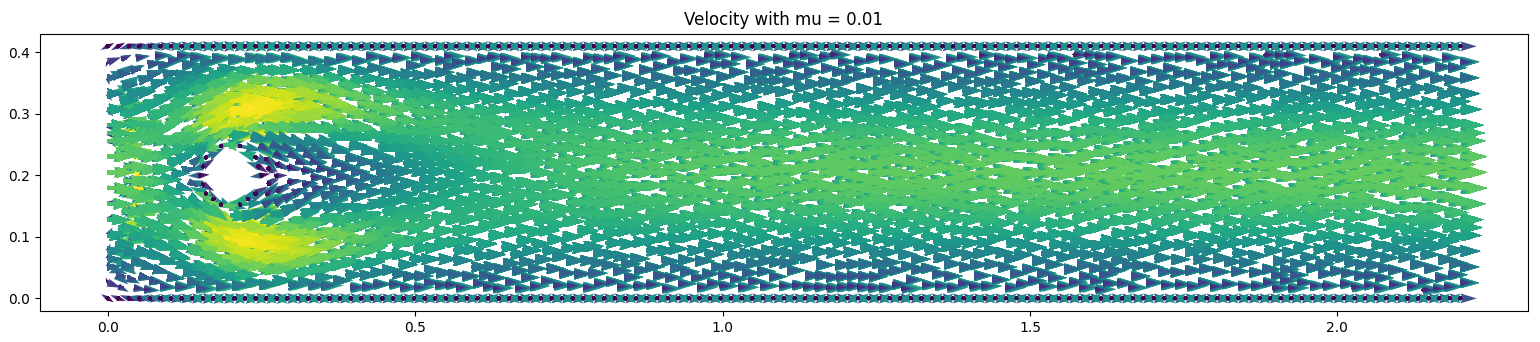
\includegraphics[width=\textwidth]{Velocity_001}
	\end{figure}
	
	\begin{figure}
		\centering
		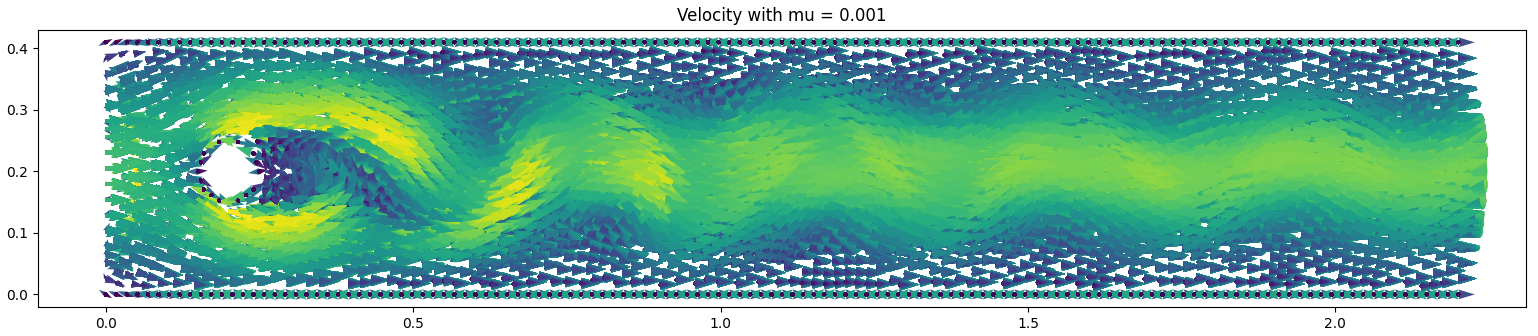
\includegraphics[width=\textwidth]{Velocity_0001}
	\end{figure}
\end{frame}

\begin{frame}
	\frametitle{Discussion}
	\textbf{Mathematics.}
	\begin{itemize}
		\item \textbf{Software for Fluids + Turbulence}: {\color{red} OpenFOAM}, Star-CCM+ (\href{https://su2code.github.io/}{SU2}, ParMooN may be later).
		\item \textbf{Turbulence}: Which turbulence models are best?
		\item Realization in the code: Topology Optimization.
		\item Need to check its physical derivation + mathematical definition of functional $\mathcal{J}_2$.
	\end{itemize}
	\textbf{Project.}
	\begin{itemize}
		\item How frequently to spend 8 months in Austria?
		\item ROMSOC - Ethical Monitoring - 3rd Assignment.
	\end{itemize}
\end{frame}

\begin{frame}
    \frametitle{Ethical Issues}
    \textbf{\color{blue} Short description of issue.}
    \begin{itemize}
        \item \textbf{ESR.} In this project, mathematical methods and software are developed for the purpose of improving combustion engines. The results could be used to improve the engine of a military vehicle after adjustments that require mathematical expert knowledge.
        \item \textbf{PI.} The developed tools can be applied to cases, where necessary conditions for a reliable output are not satisfied. This can cause misleading results, and then, wrong decisions with unintended implications.
    \end{itemize}
    \textbf{\color{blue} Strategy used to cope with it.}
    \begin{itemize}
        \item \textbf{ESR.} We will include a disclaimer, that excludes military use of the software.
        \item \textbf{PI.} Publications, preprints, technical reports are written in the course of this project. In this way, the results are explained, documented, and tested. Software tools should be well documented. The staff connected to the project is educated to understand the limits of applicability.
    \end{itemize}
\end{frame}

\begin{frame}
	\frametitle{Ethics: 7. Ongoing Monitoring. Question 1}
	{\color{blue}\bf Could you successfully implement your strategy in order to cope with the issue? (implementation of strategy)}
	\begin{itemize}
		\item \textbf{ESR.} A disclaimer excluding military use of the software will be stated in both the licence and the documentation of the software.
		\item \textbf{PI.} The implementation of the strategy can be monitored and evaluated by checking the licence and the documentation of the software. Software will be only available after contacting WIAS and signing the licence agreement.
	\end{itemize}
\end{frame}

\begin{frame}
	\frametitle{Ethics: 7. Ongoing Monitoring. Question 2}
	{\color{blue}\bf In your and your PI's opinion, is the chosen strategy working and satisfying? (evaluation of strategy: efficacy and efficiency)}
	\begin{itemize}
		\item \textbf{ESR.} Including a disclaimer in the licence and controlled access to the software are working and satisfying to prevent military use of the software.
		\item \textbf{PI.} A signed statement is an effective and efficient method and give the legal option against violators.
	\end{itemize}
\end{frame}

\begin{frame}
	\frametitle{Ethics: 7. Ongoing Monitoring. Question 3}
	{\color{blue}\bf Which are good markers, indicators and/or hints that the strategy is working a) effectively and b) efficently?}
	\begin{itemize}
		\item \textbf{ESR.} Controlled access to the software and feedback from the community by users.
		\item \textbf{PI.} Controlled access to the software and feedback from the community by users.
	\end{itemize}
\end{frame}

\begin{frame}
	\frametitle{Ethics: 7. Ongoing Monitoring. Question 4}
	{\color{blue}\bf Is there a sub-project and issue specific written and documented agreement between ESR and PI on:}
	\begin{itemize}
		\item[a)] {\color{blue}\bf how, when and by whom the strategy will be monitored until the end of the project?}
		
		\textbf{ESR.} a) The ESR writes the licence and the PI will monitor the strategy frequently during ESR's work at WIAS.
		
		\textbf{PI.} a) The ESR writes the licence and the PI will monitor the strategy frequently during ESR's work at WIAS.
	\end{itemize}
\end{frame}

\begin{frame}
	\begin{itemize}
		\item[b)] {\color{blue}\bf how the monitoring will be documented?}
		
		\textbf{ESR.} b) The PI  will monitor in exchange with the ESR the documentation of the process.
		
		\textbf{PI.} b) The PI  will monitor in exchange with the ESR the documentation of the process.
		
		\item[c)] {\color{blue}\bf how ethical monitoring after the end of the project should be assured?}
		
		\textbf{ESR.} c) The monitoring will be done by the Institute where the ESR is affiliated.
		
		\textbf{PI.} c) The monitoring will be done by the Institute where the ESR is affiliated.
	\end{itemize}
\end{frame}

\begin{frame}
	\frametitle{References}
	\begin{itemize}
		\item Maz'ya, V. and J. Rossmann (2009). \textit{Mixed boundary value problems for the stationary Navier-Stokes system in polyhedral domains}. In: Arch. Ration. Mech. Anal. 194.2, pp. 669–712.
		\item Pope, Stephen B. (2000). \textit{Turbulent flows}. Cambridge University Press, Cambridge, pp. xxxiv+771.
		\item Schmidt, Stephan (2020). \textit{Shape \& Geometry}. Humboldt University Master Course.
		\item Sokolowski, Jan and Jean-Paul Zol\'esio (1992). \textit{Introduction to shape optimization}. Vol. 16. Springer Series in Computational Mathematics. Shape sensitivity analysis. Springer-Verlag, Berlin, pp. ii+250.
		\item Temam, Roger (2000). \textit{Navier-Stokes equations. Theory and numerical analysis}. Studies in Mathematics and its Applications, Vol. 2.
		AMS Chelsea Publishing.
		\item Mohammadi, B. and O. Pironneau (1994). \textit{Analysis of the k-epsilon turbulence model}. RAM: Research in Applied Mathematics. Masson, Paris; John Wiley \& Sons, Ltd., Chichester, pp. xiv+196.
	\end{itemize}
\end{frame}

\end{document}

%%% Local Variables: 
%%% mode: latex
%%% TeX-master: t
%%% End: